\documentclass[a4paper,12pt]{article}

\usepackage[left=2.5cm, right=2.5cm, top=3cm, bottom=3cm]{geometry}
\usepackage{amsmath, amsthm, amssymb}
\usepackage[spanish]{babel}
\usepackage{cite}
\usepackage{graphicx}
\usepackage{url}
\usepackage{float}

\begin{document}
\title{Presentacion}
\author{Dario Lopez Falcon}
\date{Julio, 2023}
\maketitle


\section{Introducción}\label{sec:intro}

    Este documento fue creado con el fin de explicar como funciona el codigo de Moogle, dando a conocer sus principales
    clases y las propiedades y metodos que contien cada una de estas.
    Tambien hablaremos sobre la similitud de Cosenos y de los vectores TF y IDF ; ya que el algoritmo de busqueda de Moogle
    esta basado en estos.

\section{Clases:}\label{sec:cls}

   Es importante destacar que el codigo esta comentado en su mayoria, por lo que si quiere profundizar mas en como funciona 
 Moogle! les recomiendo que lq hechen un vistaso.

\subsection{Class Leer }\label{sub:Leer}

    El objetivo de esta clase como bien dice el nobre es leer todos los archivos .txt que se encuemtran en la base de datos , y tambien 
    guardar el nombre y el contenido de cada archivo para poder ser usados posteriormente.

    Para poder realizar estas funciones dicha clase cuenta con las propiedades y metodos que se muestran en la siguiente imagen:

\begin{figure}[H]
    \centering
    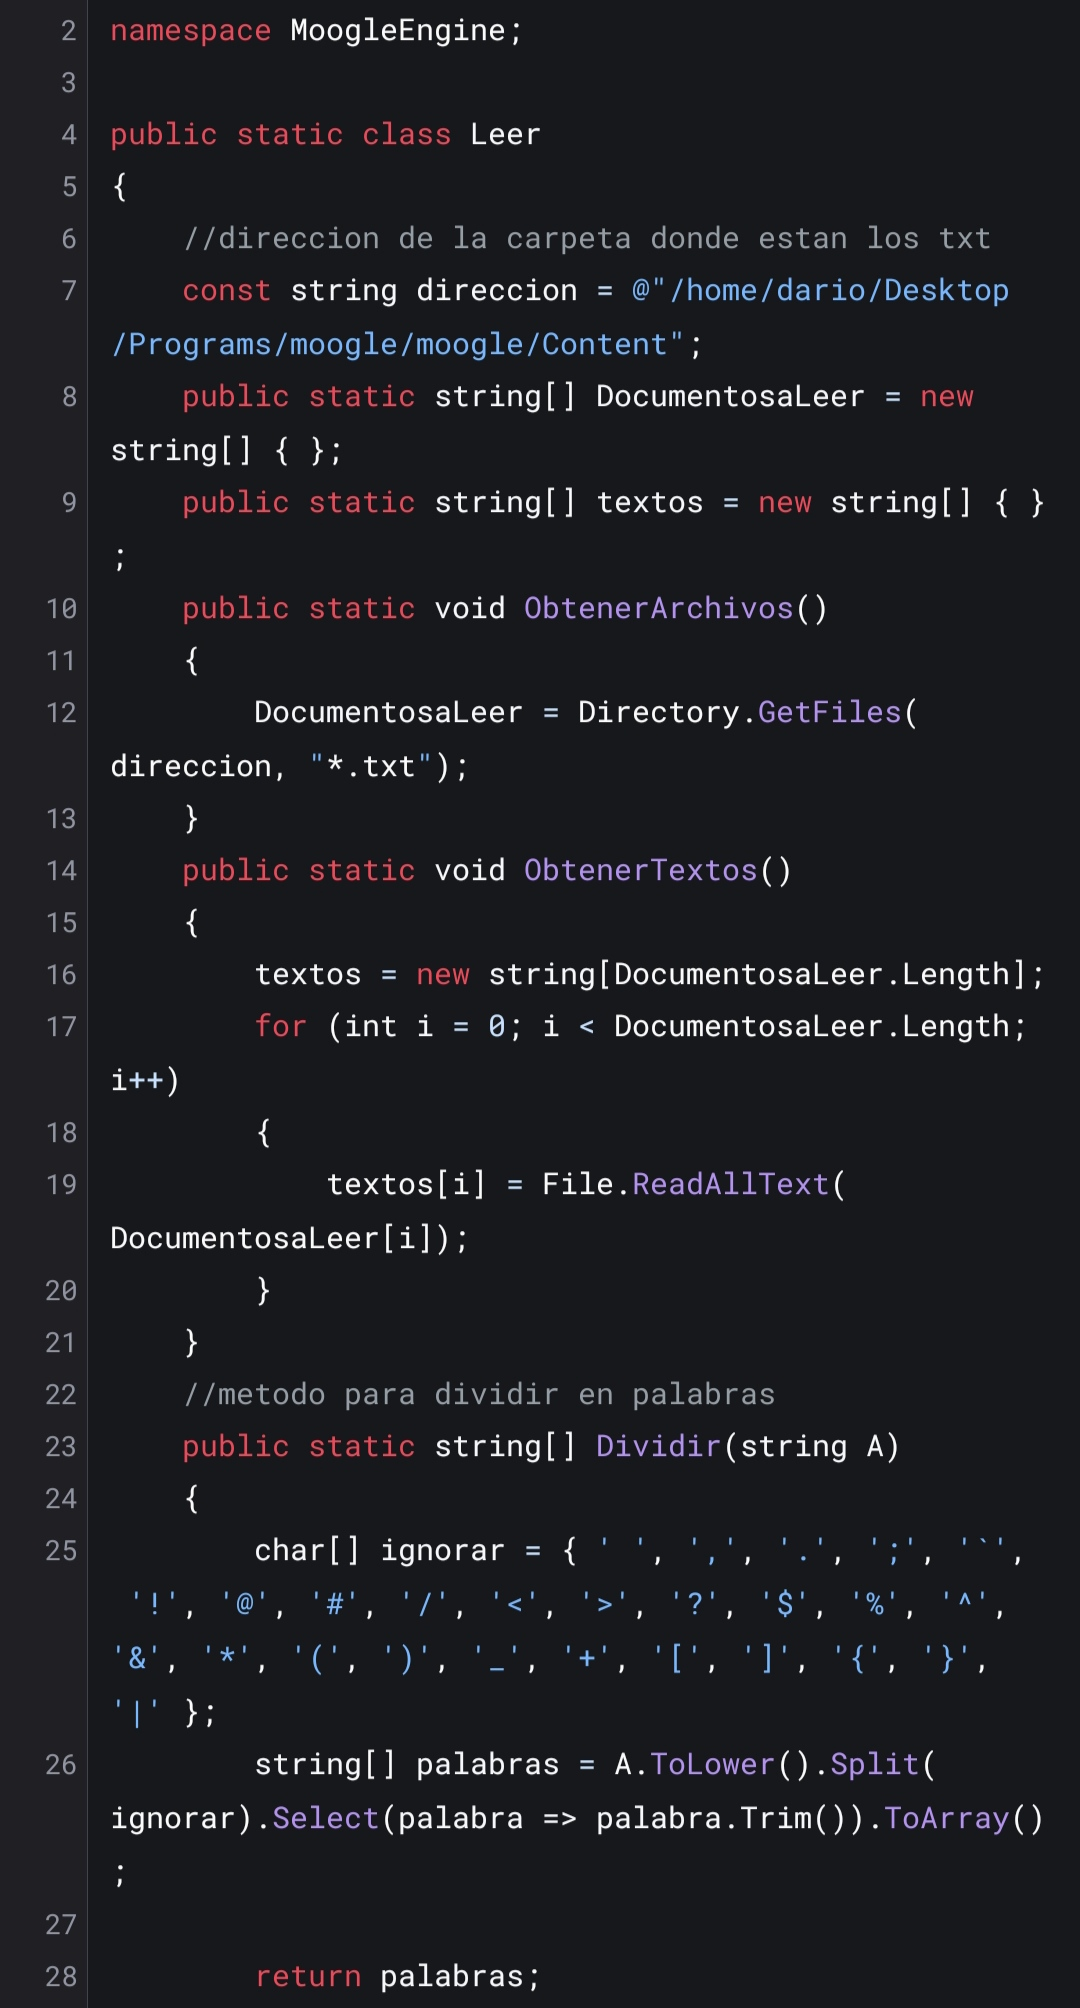
\includegraphics[width=0.25\textwidth]{imagenes/1.jpg}
\end{figure}

\subsection{Clas Documento}\label{sub:Documento}

  Por la forma en que diseñe Moogle! cada archivo de la base de datos se convertira en cun documento, se hizo indispensable
definir esta clase y darle las propiedades y metodos necesarios para la construccionde cada documento construccion de cada documento y posteriormente 
realizar la busqueda.

\begin{figure}[H]
    \centering
    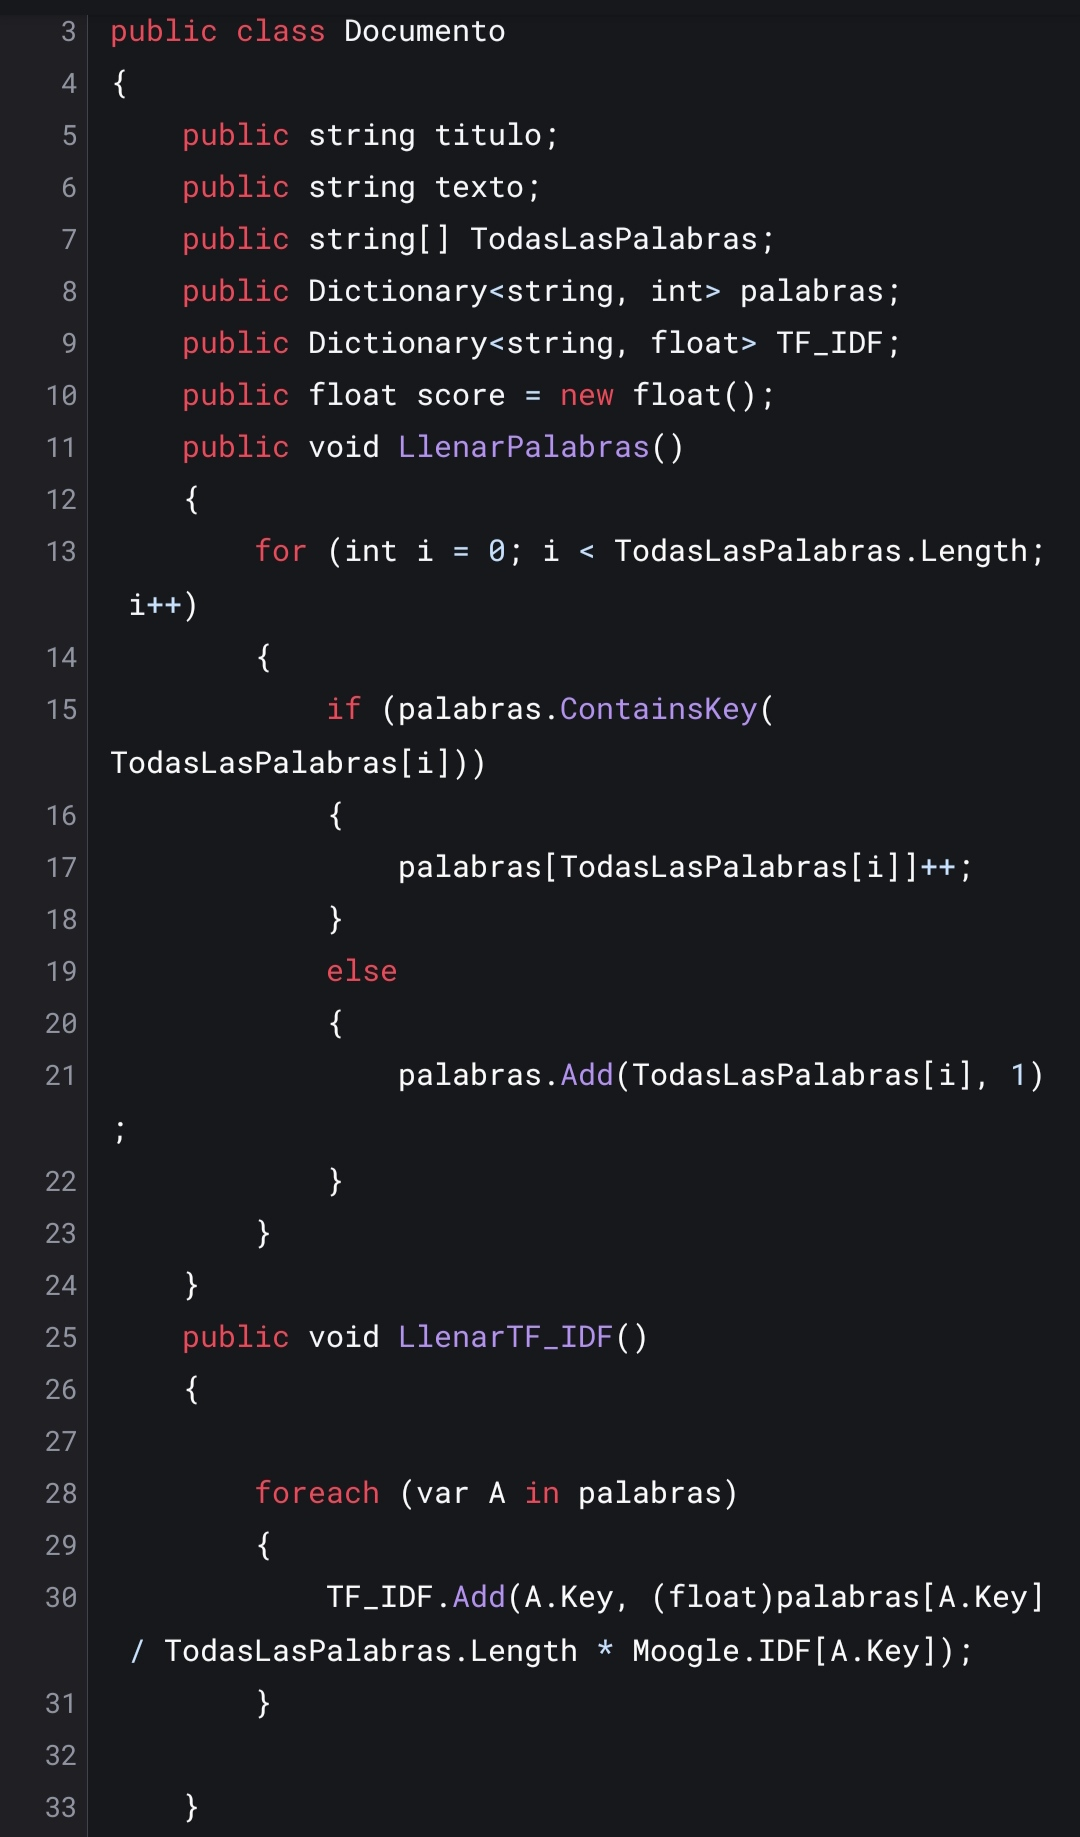
\includegraphics[width=0.25\textwidth]{imagenes/2.jpg}
\end{figure}

  Aqui ademas les dejo el constructor de la clase.

 \begin{figure}[H]
    \centering
    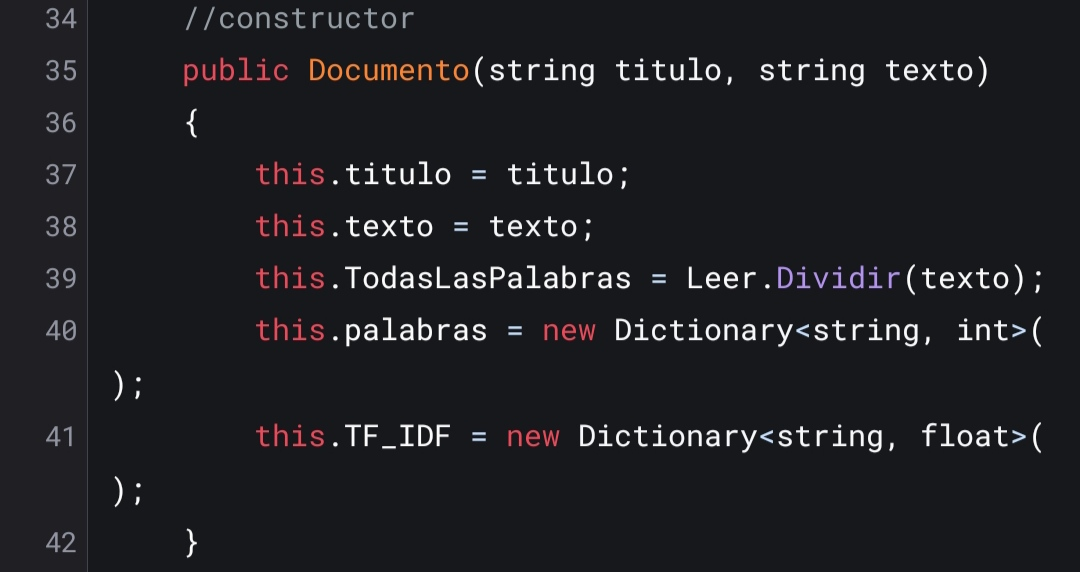
\includegraphics[width=0.25\textwidth]{imagenes/3.jpg}
\end{figure}

\subsection{Class Query}\label{sub:Query}

De manera muy similar a como es la clase Documento crearemos una nueva clase llamada Query.

\begin{figure}[H]
    \centering
    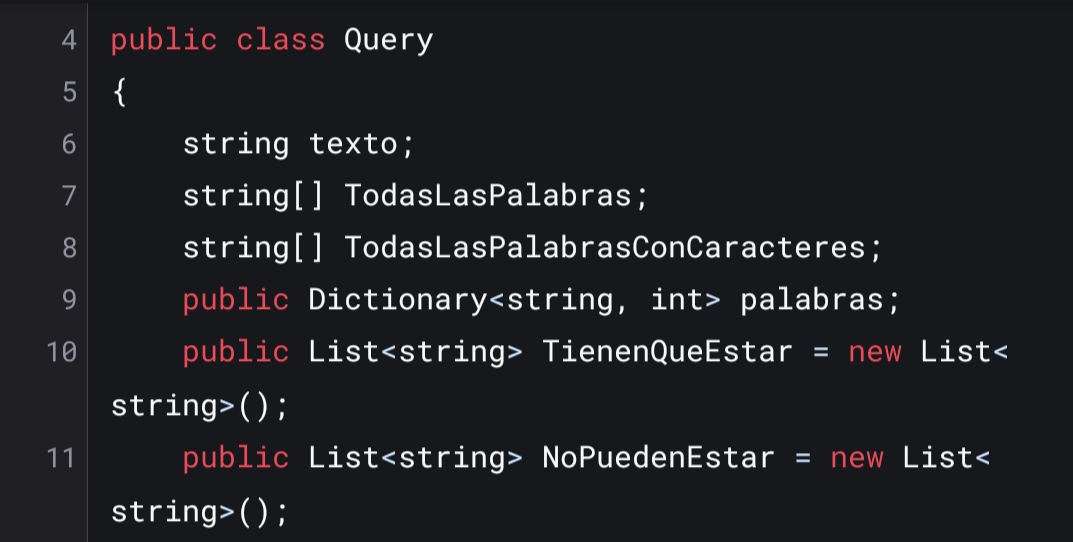
\includegraphics[width=0.5\textwidth]{imagenes/8.q.jpg}
\end{figure}

En cada busqueda convertiremos la consulta realizada en una Query .(Si desea ver los el construtor mire el codigo).

Esta clase es de vital importancia , pues en ella al igual que en cada uno de los documentos se almacena un diccionario llamado TF*IDF
que sera nuestro vector TF*IDF (del cual hablaremos mas adelante ) al cuales se le realiza la similitud de coseno con cada uno de los 
vectores TF*IDF de los documentos para asi saber que tan relevante es un documento con respecto a la Query.

En esta clase tambien podemos encontras mas metodos que son empleados para realizar busquedas mar personalizadas, a lo cual si desea saber 
en que consiste le recomiendo ver la presentacion del proyecto y posteriormente analiasar el codigo.

\subsection{Class Moogle}\label{sub:Moogle}

 Finalmente llegamos a la clase Moogle, y digo finalmente ya que es en esta clase donde se almacenan todos los metodos para contruir los documentos
 y la Query , ademas de los metodos necesarios para realizar la similitud de cosenos y organizar la salidaa.
 Pero como si todo esto fuera poco es donde se llaman y  ejecutan dichos metodos y los de las demas clases, por lo qu
 e podriamos decir que es el cuerpo
 de noestro proyecto.
 Habria quedado mas organizado creando otra clase que almacenara todos los metodos y en esta solo sean llamados para ejecutarse.

 A continuacion les dejo unas imagenes con todo lo que contiene la clase y como ya he dicho si quiere ver en porofundidad como funciona cada metodo 
 y el orden que sigo para que se ejecuten les recomiendo ver el codigo que esta comentado.

 \begin{figure}[H]
    \centering
    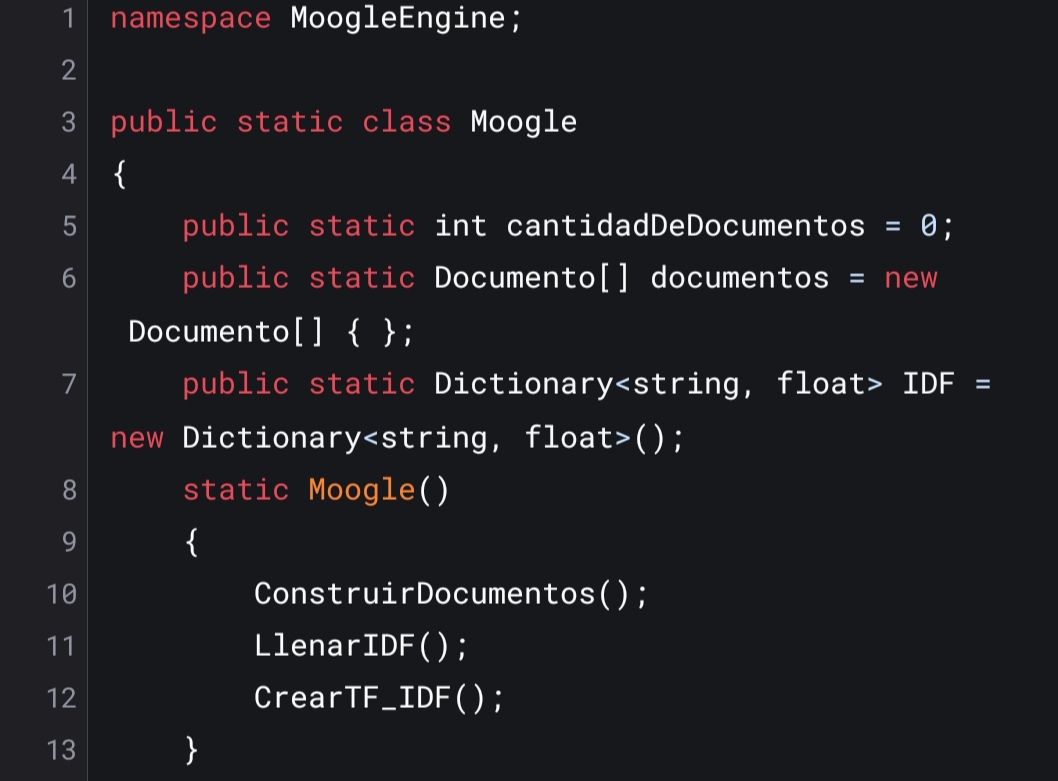
\includegraphics[width=0.6\textwidth]{imagenes/7.mo.jpg}
\end{figure}

\subsection*{Class Matrix}\label{sec:Matrix}

POr la forma en que diseñe el algoritmo de busqueda no empleo esta clase en ningun momento,pero esta forma parate del proyecto ya que esta representa una abstraccion de lo que seria una 
matriz en las matematicas, por lo que en esta clase podemos encotrar metodos que definen la suma ,el producto ,etc entre matices.

\begin{figure}[H]
    \centering
    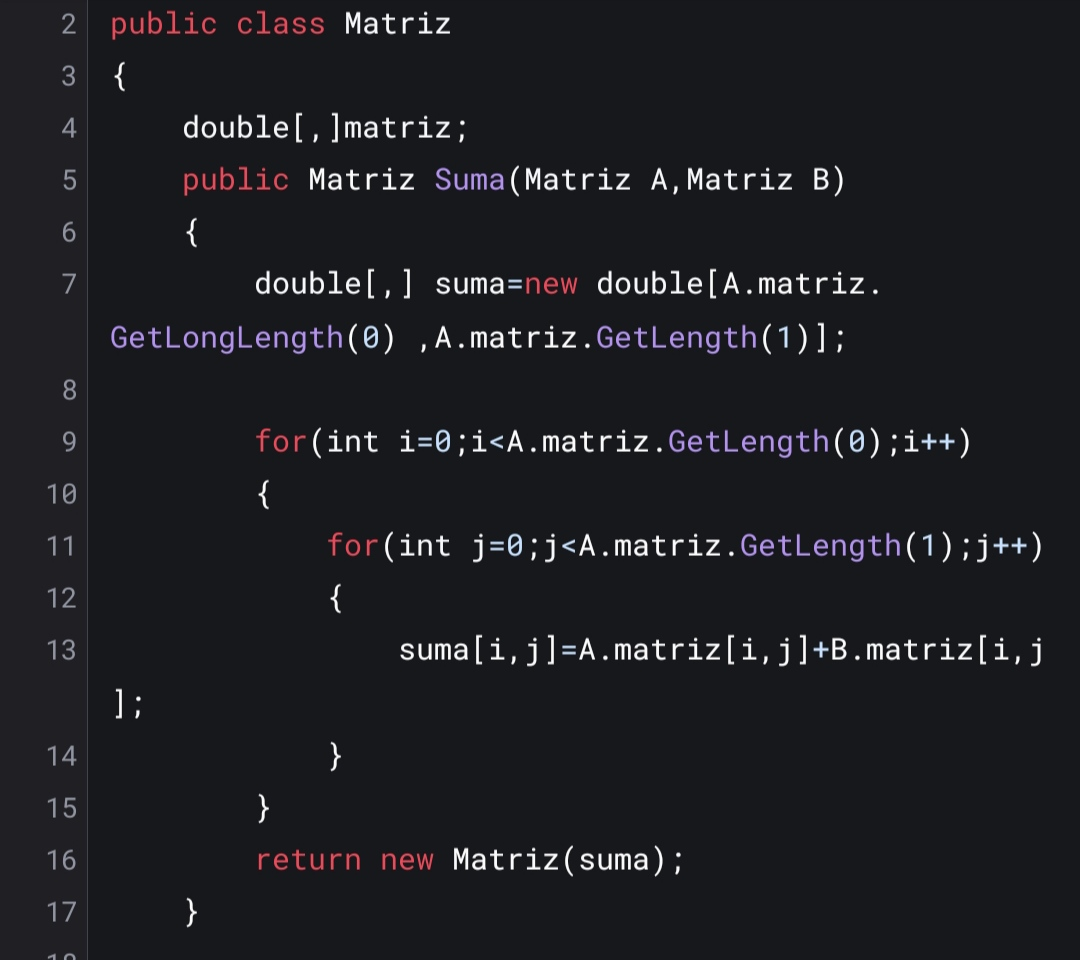
\includegraphics[width=0.5\textwidth]{imagenes/4.jpg}
\end{figure}
\begin{figure}[H]
    \centering
    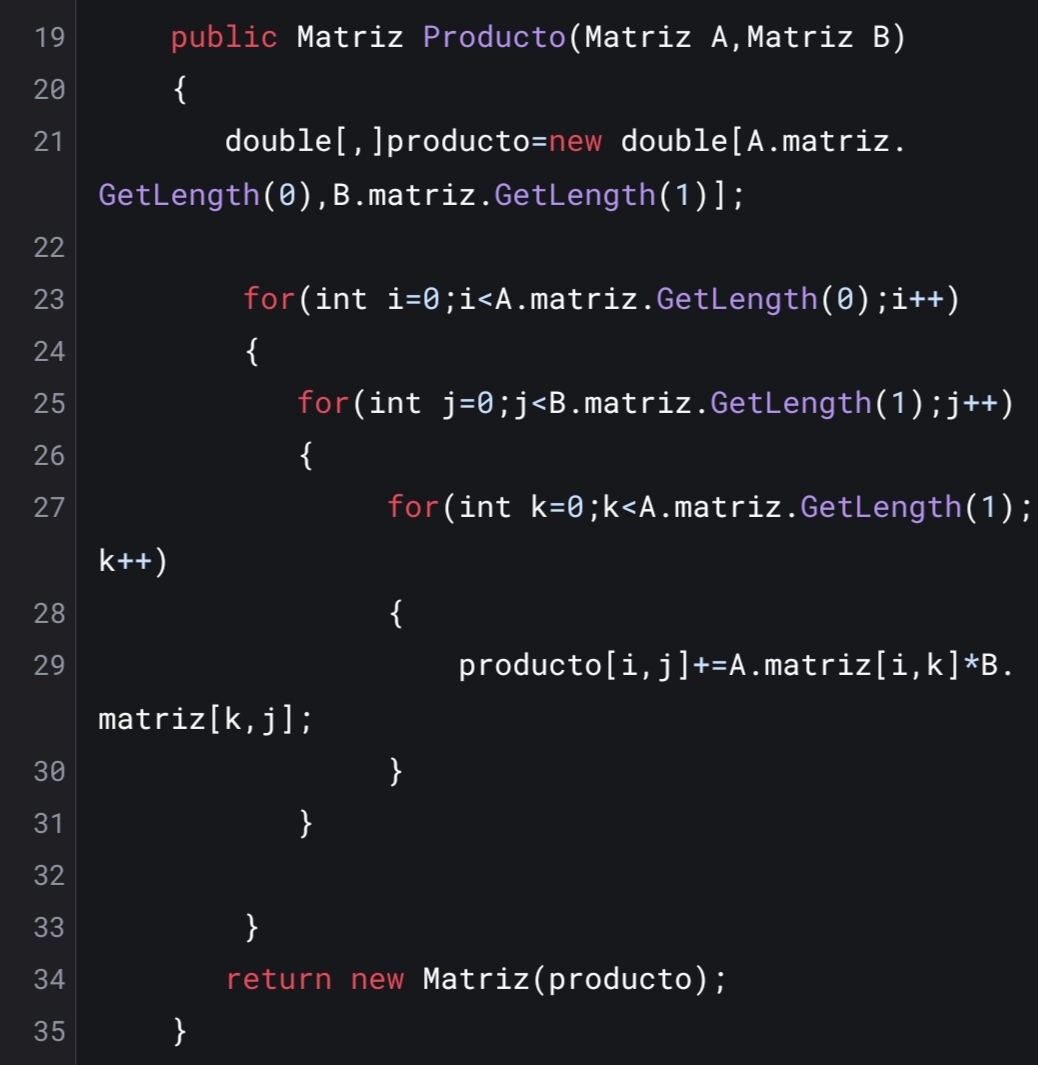
\includegraphics[width=0.5\textwidth]{imagenes/5.jpg}
\end{figure}
\begin{figure}[H]
    \centering
    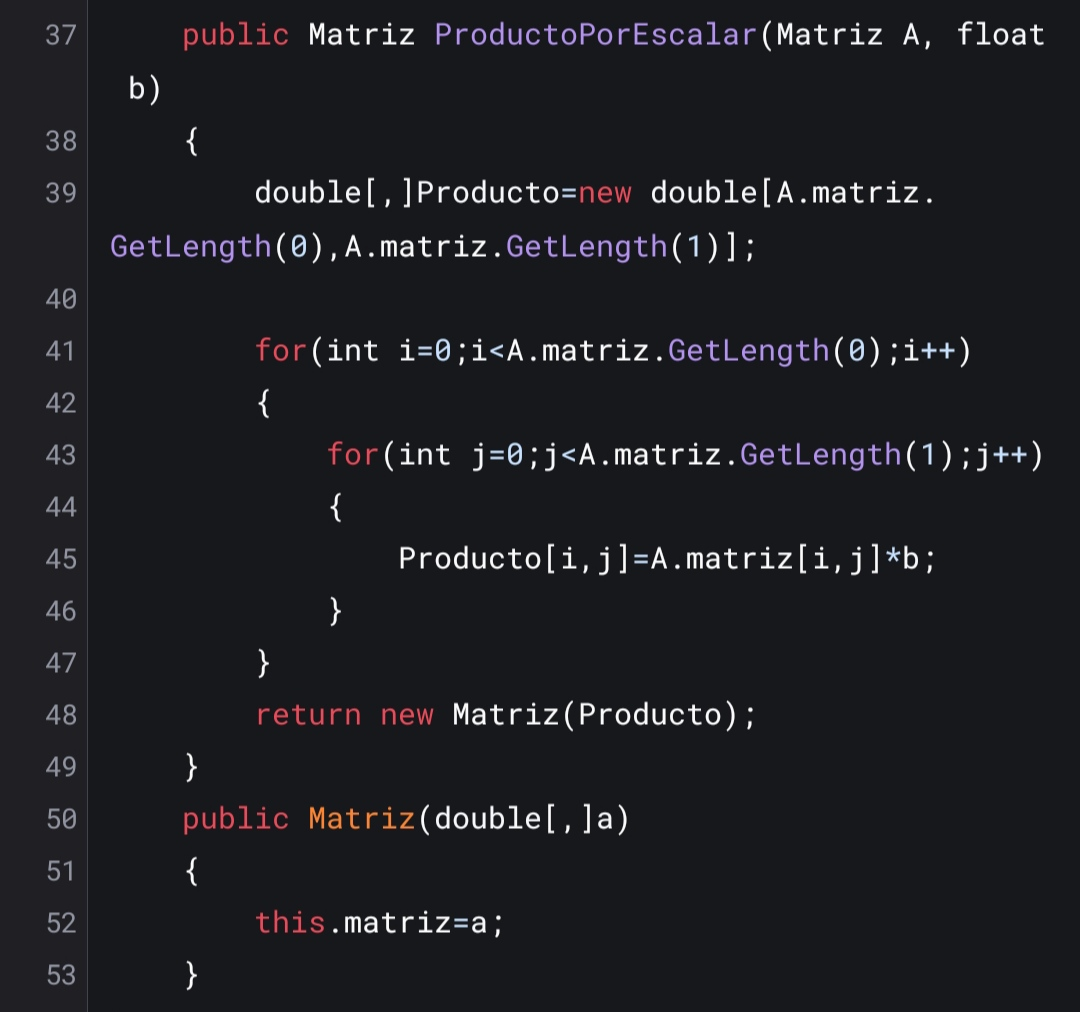
\includegraphics[width=0.5\textwidth]{imagenes/6.jpg}
\end{figure}

%\section{TF-IDF}\label{sec:TF-IDF}

%TF-IDF es una técnica utilizada en procesamiento de lenguaje natural para evaluar la relevancia de un término en un documento o corpus de textos. TF hace referencia a la frecuencia del 
%término en el documento, mientras que IDF se refiere a la frecuencia inversa del término en el corpus.

%TF (Term Frequency) mide la frecuencia con la que aparece un término en un documento específico. Cuanto mayor sea la frecuencia, más relevante se considera el término en ese documento.

%IDF (Inverse Document Frequency) mide la importancia del término en el conjunto de documentos. Calcula la frecuencia inversa para los términos que aparecen en muchos documentos, lo que 
%significa que si un término se repite en muchos documentos, su IDF será bajo y se  considerará menos relevante.

%La combinación de TF y IDF es el resultado del cálculo del producto de TF y IDF, y es utilizado para clasificar y buscar documentos en función de su relevancia en relación con un término 
%de búsqueda específico. Cuanto mayor sea el valor de TF-IDF de un término en un documento, más indicativo será su relevancia en ese documento específico.
%Luego de conocido el TF-IDF de cada documento utilizaremos para establecer una comparación entre los Documentos y la consulta un método que es muy utilizado y conocido como el método de similitud de coseno.

%\subsection{Similitud de Cosenos}\label{sub:SimilitudDeCoseno}

%El método de similitud de coseno es una técnica utilizada en minería de textos y recuperación de información para determinar cuán similar es un documento o un conjunto de palabras en relación con otro documento o conjunto de palabras. 

%Este método se basa en la idea de que la similitud entre dos vectores de características puede expresarse mediante el ángulo que forman en un espacio vectorial. En este caso, los vectores de características representan la frecuencia de las palabras en un documento (o conjunto de palabras).

%Para calcular la similitud de coseno, primero se representan los documentos o conjuntos de palabras como vectores de características. Luego, se calcula el producto punto entre estos dos vectores y se divide por el producto de las magnitudes de los vectores.

%El resultado de esta operación es un número entre -1 y 1, donde 1 indica una similitud perfecta, 0 indica que los documentos o conjuntos de palabras son completamente diferentes y -1 indica una similitud inversa.

%En resumen, el método de similitud de coseno determina la similitud entre documentos o conjuntos de palabras al operar en el espacio vectorial de características y calcular el ángulo de coseno entre ellos.

\bibliography{bibliography}
\end{document}